
%% bare_jrnl_comsoc.tex
%% V1.4b
%% 2015/08/26
%% by Michael Shell
%% see http://www.michaelshell.org/
%% for current contact information.
%%
%% This is a skeleton file demonstrating the use of IEEEtran.cls
%% (requires IEEEtran.cls version 1.8b or later) with an IEEE
%% Communications Society journal paper.
%%
%% Support sites:
%% http://www.michaelshell.org/tex/ieeetran/
%% http://www.ctan.org/pkg/ieeetran
%% and
%% http://www.ieee.org/

%%*************************************************************************
%% Legal Notice:
%% This code is offered as-is without any warranty either expressed or
%% implied; without even the implied warranty of MERCHANTABILITY or
%% FITNESS FOR A PARTICULAR PURPOSE! 
%% User assumes all risk.
%% In no event shall the IEEE or any contributor to this code be liable for
%% any damages or losses, including, but not limited to, incidental,
%% consequential, or any other damages, resulting from the use or misuse
%% of any information contained here.
%%
%% All comments are the opinions of their respective authors and are not
%% necessarily endorsed by the IEEE.
%%
%% This work is distributed under the LaTeX Project Public License (LPPL)
%% ( http://www.latex-project.org/ ) version 1.3, and may be freely used,
%% distributed and modified. A copy of the LPPL, version 1.3, is included
%% in the base LaTeX documentation of all distributions of LaTeX released
%% 2003/12/01 or later.
%% Retain all contribution notices and credits.
%% ** Modified files should be clearly indicated as such, including  **
%% ** renaming them and changing author support contact information. **
%%*************************************************************************


% *** Authors should verify (and, if needed, correct) their LaTeX system  ***
% *** with the testflow diagnostic prior to trusting their LaTeX platform ***
% *** with production work. The IEEE's font choices and paper sizes can   ***
% *** trigger bugs that do not appear when using other class files.       ***                          ***
% The testflow support page is at:
% http://www.michaelshell.org/tex/testflow/



\documentclass[journal,comsoc]{IEEEtran}
%
% If IEEEtran.cls has not been installed into the LaTeX system files,
% manually specify the path to it like:
% \documentclass[journal,comsoc]{../sty/IEEEtran}


\usepackage[T1]{fontenc}% optional T1 font encoding


% Some very useful LaTeX packages include:
% (uncomment the ones you want to load)


% *** MISC UTILITY PACKAGES ***
%
%\usepackage{ifpdf}
% Heiko Oberdiek's ifpdf.sty is very useful if you need conditional
% compilation based on whether the output is pdf or dvi.
% usage:
% \ifpdf
%   % pdf code
% \else
%   % dvi code
% \fi
% The latest version of ifpdf.sty can be obtained from:
% http://www.ctan.org/pkg/ifpdf
% Also, note that IEEEtran.cls V1.7 and later provides a builtin
% \ifCLASSINFOpdf conditional that works the same way.
% When switching from latex to pdflatex and vice-versa, the compiler may
% have to be run twice to clear warning/error messages.






% *** CITATION PACKAGES ***
%
%\usepackage{cite}
% cite.sty was written by Donald Arseneau
% V1.6 and later of IEEEtran pre-defines the format of the cite.sty package
% \cite{} output to follow that of the IEEE. Loading the cite package will
% result in citation numbers being automatically sorted and properly
% "compressed/ranged". e.g., [1], [9], [2], [7], [5], [6] without using
% cite.sty will become [1], [2], [5]--[7], [9] using cite.sty. cite.sty's
% \cite will automatically add leading space, if needed. Use cite.sty's
% noadjust option (cite.sty V3.8 and later) if you want to turn this off
% such as if a citation ever needs to be enclosed in parenthesis.
% cite.sty is already installed on most LaTeX systems. Be sure and use
% version 5.0 (2009-03-20) and later if using hyperref.sty.
% The latest version can be obtained at:
% http://www.ctan.org/pkg/cite
% The documentation is contained in the cite.sty file itself.






% *** GRAPHICS RELATED PACKAGES ***
%
\ifCLASSINFOpdf
  \usepackage[pdftex]{graphicx}
  % declare the path(s) where your graphic files are
  \graphicspath {{/Users/albertocottica/Documents/More PhD stuff/MyPhDdata/Thesis Paper 2/Paper 2 LATEX}}
  % {{../pdf/}{../jpeg/}}
  % and their extensions so you won't have to specify these with
  % every instance of \includegraphics
  % \DeclareGraphicsExtensions{.pdf,.jpeg,.png}
\else
  % or other class option (dvipsone, dvipdf, if not using dvips). graphicx
  % will default to the driver specified in the system graphics.cfg if no
  % driver is specified.
  % \usepackage[dvips]{graphicx}
  % declare the path(s) where your graphic files are
  % \graphicspath{{../eps/}}
  % and their extensions so you won't have to specify these with
  % every instance of \includegraphics
  % \DeclareGraphicsExtensions{.eps}
\fi
% graphicx was written by David Carlisle and Sebastian Rahtz. It is
% required if you want graphics, photos, etc. graphicx.sty is already
% installed on most LaTeX systems. The latest version and documentation
% can be obtained at: 
% http://www.ctan.org/pkg/graphicx
% Another good source of documentation is "Using Imported Graphics in
% LaTeX2e" by Keith Reckdahl which can be found at:
% http://www.ctan.org/pkg/epslatex
%
% latex, and pdflatex in dvi mode, support graphics in encapsulated
% postscript (.eps) format. pdflatex in pdf mode supports graphics
% in .pdf, .jpeg, .png and .mps (metapost) formats. Users should ensure
% that all non-photo figures use a vector format (.eps, .pdf, .mps) and
% not a bitmapped formats (.jpeg, .png). The IEEE frowns on bitmapped formats
% which can result in "jaggedy"/blurry rendering of lines and letters as
% well as large increases in file sizes.
%
% You can find documentation about the pdfTeX application at:
% http://www.tug.org/applications/pdftex





% *** MATH PACKAGES ***
%
\usepackage{amsmath}
% A popular package from the American Mathematical Society that provides
% many useful and powerful commands for dealing with mathematics.
% Do NOT use the amsbsy package under comsoc mode as that feature is
% already built into the Times Math font (newtxmath, mathtime, etc.).
% 
% Also, note that the amsmath package sets \interdisplaylinepenalty to 10000
% thus preventing page breaks from occurring within multiline equations. Use:
\interdisplaylinepenalty=2500
% after loading amsmath to restore such page breaks as IEEEtran.cls normally
% does. amsmath.sty is already installed on most LaTeX systems. The latest
% version and documentation can be obtained at:
% http://www.ctan.org/pkg/amsmath


% Select a Times math font under comsoc mode or else one will automatically
% be selected for you at the document start. This is required as Communications
% Society journals use a Times, not Computer Modern, math font.
\usepackage[cmintegrals]{newtxmath}
% The freely available newtxmath package was written by Michael Sharpe and
% provides a feature rich Times math font. The cmintegrals option, which is
% the default under IEEEtran, is needed to get the correct style integral
% symbols used in Communications Society journals. Version 1.451, July 28,
% 2015 or later is recommended. Also, do *not* load the newtxtext.sty package
% as doing so would alter the main text font.
% http://www.ctan.org/pkg/newtx
%
% Alternatively, you can use the MathTime commercial fonts if you have them
% installed on your system:
%\usepackage{mtpro2}
%\usepackage{mt11p}
%\usepackage{mathtime}


%\usepackage{bm}
% The bm.sty package was written by David Carlisle and Frank Mittelbach.
% This package provides a \bm{} to produce bold math symbols.
% http://www.ctan.org/pkg/bm





% *** SPECIALIZED LIST PACKAGES ***
%
%\usepackage{algorithmic}
% algorithmic.sty was written by Peter Williams and Rogerio Brito.
% This package provides an algorithmic environment fo describing algorithms.
% You can use the algorithmic environment in-text or within a figure
% environment to provide for a floating algorithm. Do NOT use the algorithm
% floating environment provided by algorithm.sty (by the same authors) or
% algorithm2e.sty (by Christophe Fiorio) as the IEEE does not use dedicated
% algorithm float types and packages that provide these will not provide
% correct IEEE style captions. The latest version and documentation of
% algorithmic.sty can be obtained at:
% http://www.ctan.org/pkg/algorithms
% Also of interest may be the (relatively newer and more customizable)
% algorithmicx.sty package by Szasz Janos:
% http://www.ctan.org/pkg/algorithmicx




% *** ALIGNMENT PACKAGES ***
%
\usepackage{array}
% Frank Mittelbach's and David Carlisle's array.sty patches and improves
% the standard LaTeX2e array and tabular environments to provide better
% appearance and additional user controls. As the default LaTeX2e table
% generation code is lacking to the point of almost being broken with
% respect to the quality of the end results, all users are strongly
% advised to use an enhanced (at the very least that provided by array.sty)
% set of table tools. array.sty is already installed on most systems. The
% latest version and documentation can be obtained at:
% http://www.ctan.org/pkg/array


% IEEEtran contains the IEEEeqnarray family of commands that can be used to
% generate multiline equations as well as matrices, tables, etc., of high
% quality.




% *** SUBFIGURE PACKAGES ***
%\ifCLASSOPTIONcompsoc
%  \usepackage[caption=false,font=normalsize,labelfont=sf,textfont=sf]{subfig}
%\else
%  \usepackage[caption=false,font=footnotesize]{subfig}
%\fi
% subfig.sty, written by Steven Douglas Cochran, is the modern replacement
% for subfigure.sty, the latter of which is no longer maintained and is
% incompatible with some LaTeX packages including fixltx2e. However,
% subfig.sty requires and automatically loads Axel Sommerfeldt's caption.sty
% which will override IEEEtran.cls' handling of captions and this will result
% in non-IEEE style figure/table captions. To prevent this problem, be sure
% and invoke subfig.sty's "caption=false" package option (available since
% subfig.sty version 1.3, 2005/06/28) as this is will preserve IEEEtran.cls
% handling of captions.
% Note that the Computer Society format requires a larger sans serif font
% than the serif footnote size font used in traditional IEEE formatting
% and thus the need to invoke different subfig.sty package options depending
% on whether compsoc mode has been enabled.
%
% The latest version and documentation of subfig.sty can be obtained at:
% http://www.ctan.org/pkg/subfig




% *** FLOAT PACKAGES ***
%
%\usepackage{fixltx2e}
% fixltx2e, the successor to the earlier fix2col.sty, was written by
% Frank Mittelbach and David Carlisle. This package corrects a few problems
% in the LaTeX2e kernel, the most notable of which is that in current
% LaTeX2e releases, the ordering of single and double column floats is not
% guaranteed to be preserved. Thus, an unpatched LaTeX2e can allow a
% single column figure to be placed prior to an earlier double column
% figure.
% Be aware that LaTeX2e kernels dated 2015 and later have fixltx2e.sty's
% corrections already built into the system in which case a warning will
% be issued if an attempt is made to load fixltx2e.sty as it is no longer
% needed.
% The latest version and documentation can be found at:
% http://www.ctan.org/pkg/fixltx2e


\usepackage{stfloats}
% stfloats.sty was written by Sigitas Tolusis. This package gives LaTeX2e
% the ability to do double column floats at the bottom of the page as well
% as the top. (e.g., "\begin{figure*}[!b]" is not normally possible in
% LaTeX2e). It also provides a command:
%\fnbelowfloat
% to enable the placement of footnotes below bottom floats (the standard
% LaTeX2e kernel puts them above bottom floats). This is an invasive package
% which rewrites many portions of the LaTeX2e float routines. It may not work
% with other packages that modify the LaTeX2e float routines. The latest
% version and documentation can be obtained at:
% http://www.ctan.org/pkg/stfloats
% Do not use the stfloats baselinefloat ability as the IEEE does not allow
% \baselineskip to stretch. Authors submitting work to the IEEE should note
% that the IEEE rarely uses double column equations and that authors should try
% to avoid such use. Do not be tempted to use the cuted.sty or midfloat.sty
% packages (also by Sigitas Tolusis) as the IEEE does not format its papers in
% such ways.
% Do not attempt to use stfloats with fixltx2e as they are incompatible.
% Instead, use Morten Hogholm'a dblfloatfix which combines the features
% of both fixltx2e and stfloats:
%
% \usepackage{dblfloatfix}
% The latest version can be found at:
% http://www.ctan.org/pkg/dblfloatfix




%\ifCLASSOPTIONcaptionsoff
%  \usepackage[nomarkers]{endfloat}
% \let\MYoriglatexcaption\caption
% \renewcommand{\caption}[2][\relax]{\MYoriglatexcaption[#2]{#2}}
%\fi
% endfloat.sty was written by James Darrell McCauley, Jeff Goldberg and 
% Axel Sommerfeldt. This package may be useful when used in conjunction with 
% IEEEtran.cls'  captionsoff option. Some IEEE journals/societies require that
% submissions have lists of figures/tables at the end of the paper and that
% figures/tables without any captions are placed on a page by themselves at
% the end of the document. If needed, the draftcls IEEEtran class option or
% \CLASSINPUTbaselinestretch interface can be used to increase the line
% spacing as well. Be sure and use the nomarkers option of endfloat to
% prevent endfloat from "marking" where the figures would have been placed
% in the text. The two hack lines of code above are a slight modification of
% that suggested by in the endfloat docs (section 8.4.1) to ensure that
% the full captions always appear in the list of figures/tables - even if
% the user used the short optional argument of \caption[]{}.
% IEEE papers do not typically make use of \caption[]'s optional argument,
% so this should not be an issue. A similar trick can be used to disable
% captions of packages such as subfig.sty that lack options to turn off
% the subcaptions:
% For subfig.sty:
% \let\MYorigsubfloat\subfloat
% \renewcommand{\subfloat}[2][\relax]{\MYorigsubfloat[]{#2}}
% However, the above trick will not work if both optional arguments of
% the \subfloat command are used. Furthermore, there needs to be a
% description of each subfigure *somewhere* and endfloat does not add
% subfigure captions to its list of figures. Thus, the best approach is to
% avoid the use of subfigure captions (many IEEE journals avoid them anyway)
% and instead reference/explain all the subfigures within the main caption.
% The latest version of endfloat.sty and its documentation can obtained at:
% http://www.ctan.org/pkg/endfloat
%
% The IEEEtran \ifCLASSOPTIONcaptionsoff conditional can also be used
% later in the document, say, to conditionally put the References on a 
% page by themselves.




% *** PDF, URL AND HYPERLINK PACKAGES ***
%
%\usepackage{url}
% url.sty was written by Donald Arseneau. It provides better support for
% handling and breaking URLs. url.sty is already installed on most LaTeX
% systems. The latest version and documentation can be obtained at:
% http://www.ctan.org/pkg/url
% Basically, \url{my_url_here}.




% *** Do not adjust lengths that control margins, column widths, etc. ***
% *** Do not use packages that alter fonts (such as pslatex).         ***
% There should be no need to do such things with IEEEtran.cls V1.6 and later.
% (Unless specifically asked to do so by the journal or conference you plan
% to submit to, of course. )


% correct bad hyphenation here
\hyphenation{op-tical net-works semi-conduc-tor}


\begin{document}
%
% paper title
% Titles are generally capitalized except for words such as a, an, and, as,
% at, but, by, for, in, nor, of, on, or, the, to and up, which are usually
% not capitalized unless they are the first or last word of the title.
% Linebreaks \\ can be used within to get better formatting as desired.
% Do not put math or special symbols in the title.
\title{Bare Demo of IEEEtran.cls for\\ IEEE Communications Society Journals}
%
%
% author names and IEEE memberships
% note positions of commas and nonbreaking spaces ( ~ ) LaTeX will not break
% a structure at a ~ so this keeps an author's name from being broken across
% two lines.
% use \thanks{} to gain access to the first footnote area
% a separate \thanks must be used for each paragraph as LaTeX2e's \thanks
% was not built to handle multiple paragraphs
%

\author{Alberto Cottica}% <-this % stops a space
\thanks{Thanks go here.}% <-this % stops a space
\thanks{Manuscript received April 19, 2005; revised August 26, 2015.}}

% note the % following the last \IEEEmembership and also \thanks - 
% these prevent an unwanted space from occurring between the last author name
% and the end of the author line. i.e., if you had this:
% 
% \author{....lastname \thanks{...} \thanks{...} }
%                     ^------------^------------^----Do not want these spaces!
%
% a space would be appended to the last name and could cause every name on that
% line to be shifted left slightly. This is one of those "LaTeX things". For
% instance, "\textbf{A} \textbf{B}" will typeset as "A B" not "AB". To get
% "AB" then you have to do: "\textbf{A}\textbf{B}"
% \thanks is no different in this regard, so shield the last } of each \thanks
% that ends a line with a % and do not let a space in before the next \thanks.
% Spaces after \IEEEmembership other than the last one are OK (and needed) as
% you are supposed to have spaces between the names. For what it is worth,
% this is a minor point as most people would not even notice if the said evil
% space somehow managed to creep in.



% The paper headers
%\markboth{Journal of \LaTeX\ Class Files,~Vol.~14, No.~8, August~2015}%
%{Shell \MakeLowercase{\textit{et al.}}: Bare Demo of IEEEtran.cls for IEEE Communications Society Journals}
% The only time the second header will appear is for the odd numbered pages
% after the title page when using the twoside option.
% 
% *** Note that you probably will NOT want to include the author's ***
% *** name in the headers of peer review papers.                   ***
% You can use \ifCLASSOPTIONpeerreview for conditional compilation here if
% you desire.




% If you want to put a publisher's ID mark on the page you can do it like
% this:
%\IEEEpubid{0000--0000/00\$00.00~\copyright~2015 IEEE}
% Remember, if you use this you must call \IEEEpubidadjcol in the second
% column for its text to clear the IEEEpubid mark.



% use for special paper notices
%\IEEEspecialpapernotice{(Invited Paper)}




% make the title area
\maketitle
Microfoundations of online community management: some empirical evidence
% As a general rule, do not put math, special symbols or citations
% in the abstract or keywords.
\begin{abstract}
The abstract goes here.
\end{abstract}

% Note that keywords are not normally used for peerreview papers.
%\begin{IEEEkeywords}
%Communications Society, IEEE, IEEEtran, journal, \LaTeX, paper, template.
%\end{IEEEkeywords}






% For peer review papers, you can put extra information on the cover
% page as needed:
% \ifCLASSOPTIONpeerreview
% \begin{center} \bfseries EDICS Category: 3-BBND \end{center}
% \fi
%
% For peerreview papers, this IEEEtran command inserts a page break and
% creates the second title. It will be ignored for other modes.
\IEEEpeerreviewmaketitle

-\section{Introduction}

Online communities are used to aggregate and process information dispersed across many individuals. Pioneered in the 1980s, they have become more widespread with mass adoption of the Internet, and are now used across many different contexts in business \cite{mcwilliam2012building, tapscott2008wikinomics}, politics and public decision making \cite{rheingold1993virtual, noveck2009wiki, cottica2010wikicrazia}, expertise sharing \cite{rheingold1993virtual, zhang2007expertise, shirky2008here}, and education \cite{milligan2013patterns}. At the same time as they spread across domains, they did so geographically: for example, they have attracted large numbers of users and large venture capital investments in China \cite{zhou2011social}. Most online communities lack a central command structure; despite this, many display remarkably coherent behaviour, and have proven effective at large tasks like writing the largest encyclopedia in human history (Wikipedia), providing an always-on free helpline for software engineering problems (StackOverflow), or building, and continuously updating, a detailed map of planet Earth (OpenStreetMap) \cite{shirky2008here}. 

Organizations running online communities typically employ community managers, tasked with encouraging participation and resolving conflict: this practice is almost as old as online communities themselves and predates the Internet \cite{rheingold1993virtual}, although it has become much more widespread as Internet access became a mass phenomenon. Though most participants to online communities are unpaid and answer to no one, a small number of them (only one or two in the smaller communities, many more in the larger ones) report to a central command, and carry out its directives. Following the convention of practitioners themselves, we shall henceforth call such directives \emph{policies}. 

Putting in place policies for online communities is costly. Professional community managers need to be recruited, trained and paid; software tools to monitor communities and make their work possible need to be developed and maintained. This raises the question of what benefits organisations running online communities expect from policies; and why they choose certain policies, and not others. 

A full investigation of this matter is outside the scope of this paper; however, in what follows we outline and briefly discuss the set of assumptions that underpin our investigation. 

\begin{enumerate}
\item In line with the network science approach to online communities, we model online communities as social networks of interactions across participants. 
\item We assume that organisations can be modelled as economic agents maximising some objective function. The target variable being maximised can be profit (for online communities run by commercial companies); or welfare (for online communities run by governments or other nonprofit entities); or some combination of the two. 
\item We assume that the topology of the interaction network characteristic of online communities affects their ability to contribute to the maximisation of the target variable. 
\item We assume that such organisations choose their policies as follows: 
\begin{itemize} 
	\item Solve their maximisation problem over network topology. This yields a vector of desired network characteristics, where "desired" means that those characteristics define a maximum of the objective function. These solutions will be statements with the form "In order to best meet our ultimate [profit or welfare] goals, the interaction network in our online community should be in state $\Theta_D$, where $\Theta$ is a vector of topology-related parameters".
	\item Derive a course of action that community managers could take to change the network away from its present state $\Theta_0$ to the desired state $\Theta_D$.
	\item Encode such course of action in a set of simple instructions for community managers to execute. They call them policies;  computer scientists might think of such instructions as algorithms; economists call them mechanisms. 
\end{itemize}
\end{enumerate}

All this implies that the organisation running the online community has tools at its disposal to (attempt to) reach such preferred states of the interaction network. But rarely, if ever, is it explicitly argued that, in fact, it does. Network topology results from the uncoordinated behaviour of all users of the online community. Most of them have joined the community by their own free will, can leave at any time, and can in no way be forced to comply with the organisation's directives. This makes topology an emergent property of the pattern of interaction. For recommendations about "better" states to be meaningful, we need to verify that organisations have the tools to achieve them. 

This paper attempts to bridge that gap. To do so, it does not attempt to model the whole chain of decision starting from the maximisation problem. Rather, it focuses on those participants in an online community that \textit{are} answerable to the organisation in charge of it: its online community managers. We conjecture the following:

\begin{enumerate}
 	\item Organisations can formulate policies and instruct online community managers to execute them.
	 \item Online community managers execute by communicating with users.
	 \item Communication with online community managers nudges users towards taking the course of action desired by the organisation. 
 \end{enumerate}
 
The first two items in this list are assumed to fit into the mechanism design framework. This entails assuming that the organisation in charge of the online community knows both the desired network state $\Theta_D$ and the set of behaviours that, were they adopted by the online community's users, would result in it achieving $\Theta_D$. We focus on the final item, which is equivalent to assuming that user behaviour is responsive to communication with online community managers. This assumption is implicit both in the literature and in managerial practice but, to the best of our knowledge, has not yet been tested.

We consider a policy aimed at user activation: it consists of commenting a unit of content authored by a user. The comment could read something like the one below:

\emph{``Hello, Alice! That was a very interesting point. It definitely resonates with my own experience in the field. In our community, the people who are most involved in the matter are Bob [link] and Charlie [link]. You might be interested in this post [link] by Bob, where he relates his own experience: if you leave him a comment, I am sure an interesting conversation will ensue.''}

It is successful if the user becomes active in the current period.  

Many online communities take care to do this systematically with new users. As a new participant becomes active (for example by posting her first post, or commenting somebody else's post for the first time), community managers are instructed to leave her a comment that contains (a) friendly, positive feedback and (b) suggestions to engage with other, existing participants that she might have interests in common with,\footnote{Katherina Fake, founder of Flickr, a popular website to share photographs, is reported to have deployed the company's employees as the website's first users and the initial core of its community. According to her "We learned you have to greet the first ten thousand users personally". \cite{shirky2008here}} perhaps one of the simplest and most common in online community management \cite{rheingold1993virtual, shirky2008here}. 

In the remainder of the paper, we consider the issue of whether user behaviour does, indeed, respond to activation policies. Organizations running online communities invest considerable resources in them, and user responsiveness is an important parameter in making the decision of how much to spend in this activity as opposed to other, competing ones.  

Section 2 briefly examines the literature that we mostly draw upon. Section 3 presents some data from a real-world online community called Edgeryders; then proceeds to specify a model of that community's user behaviour in the presence of activation policies. Section 4 presents the estimation's results. Section 5 discusses them.
 -\section{Literature survey}

We are interested in the responsiveness of the behaviour of participants in online communities when policies, aiming to change the topology of the interaction network to a desired state, are enacted by the organisations in charge of the online community itself. This topic finds itself at the intersection of two different strands of academic literature.

The first strand is mainly interested in the determinants of the behaviour of individuals participating in online communities. Many scholars, moving from a psychology or business management background, take the view that individual behaviour in online community both responds to social norms and contributes to shape them. Several attempts have been made to conceptualize this view into testable models (\cite{armstrong2000real}, \cite{dholakia2004social}, \cite{zhou2011social}). Such attempts use survey data to estimate structural equation models. The models' parameters quantify the influence of both individual incentives (such as obtaining valued information) and social incentives (such as group norms) in participating in online communities. 

The second strand moves from a social network science background, and focuses on the interplay between network topology and user behaviour. The best-known example is probably Ronald Burt's theory of structural holes (\cite{burt2005brokerage}), which generalises to any community, both online and offline. There exist several studies dedicated to specific online communities, such as Slashdot (\cite{toral2009empirical}), Java developers forums (\cite{zhang2007expertise}) and Linux ports developer forums (\cite{ganley2009ties}). Some authors have attempted to merge these two strands of literature, treating network topology characteristics as variables to incorporate into their structural equation models (\cite{toral2009empirical}, \cite{ganley2009ties}).

Authors from both strands agree that some topological characteristics are more conducive than others to the organisation's goals. For example, Burt (\cite{burt2005brokerage}) suggests that densely connected clusters of individuals are useful to better focus on goals and targets, whereas less dense networks with some individuals bridging across clusters are more conducive to innovation; Ganley and Lampe (\cite{ganley2009ties}) propose that densely connected clusters of "power users" lead to social tensions and a loss of the egalitarian spirit that makes many online communities attractive; Kim and collaborators (\cite{kim2015group}) show that, in some circumstances, a tendency towards communication reciprocity ("intimacy") leads to membership loss and, potentially, network breakdown. Dholakia and collaborators are perhaps clearest in indicating that their findings are relevant to designing and enacting policies:

\begin{quotation}
Understanding the antecedents of social influence is important since it is likely to provide significant managerial guidance regarding how to make virtual communities useful and influential for their participants. (\cite{dholakia2004social}, p. 242) 
\end{quotation}

Most authors do not explicitly envision pathways leading from the formulation of a policy to attaining the desired change in network topology. Some do point to the relevance of online community managers, explicitly (\cite{dholakia2004social}) or implicitly (\cite{toral2009empirical}), by referring to cases in which such professionals are prominent (\cite{rheingold1993virtual}); but we have been unable to find an explicit discussion of how few online community manager can wilfully alter the behaviour of the many participants to the same community. Departing from this practice, in a previous paper (\cite{cottica2015online}), we have proposed such a pathway for the onboarding policy: online community managers communicate one-to-one with new members of the online community and suggest they initiate communication with existing members, indicating those existing members that seem to match the newcomer's interests best. This paper provides an empirical test that such behaviour does indeed prompt users to interact with each other, underpinning the usefulness and profitability of engaging in online community management activities.  

The present paper is also related to the growing mass of literature on the treatment of time in network analysis. Early work in networks, both in mathematics (for example \cite{erdds1959random}) and in sociology (for example \cite{moreno1937sociometry}), focused on the topology of static networks. The beginning of the 21st century marked a surge of interest in evolving networks (for example \cite{barabasi1999emergence} and related work; see \cite{dorogovtsev2002evolution} for a survey). Scholars sharing this interest investigate the growth paths that produce certain notable topologies often encountered in real-world networks. Later still, a literature on dynamic networks developed, interested in dynamical processes that happen in networks, like information diffusion (for example \cite{eckmann2004entropy}) or epidemics (for example \cite{rocha2011simulated}). Many of these studies direct their attention towards the statistical properties of the sequences of event that make up spreading dynamics. Human communication dynamics, they find, turns out to be "bursty", with the timings between communication events deviating significantly from uniform or Poissonian statistics  (see \cite{holme2012temporal} for a survey). 

Our focus does not lie in the dynamics of communication events in online communities. Rather, we wish to establish whether  community managers can really influence the behaviour of participants in the online community. The pattern of relationships across the community is likely to have some influence on users' willingness to initiate communication. Since such patterns varies across time, we adopt the stance of representing temporal data as a sequence of static graphs, tracing the evolution of the interaction network. This allows us to treat the topology of the network as a control variable, whose effect on the users likelihood to initiate communication must be kept separate from that of the action of community managers. This technique, while entailing a loss of information, is deemed appropriate when, as is our case, topology is more central to the analysis than time sequence (\cite{rosvall2010mapping}).

 -\section{Materials and methods}

\subsection{Data}

We consider an online community called Edgeryders, whose members discuss and try to implement various projects connected to social innovation in a decentralized manner. The community is run by a British company, also called Edgeryders, which we cast as the policy maker of the community. The affordances of the online platform that hosts the community and its discussion deeply influence the social dynamics thereof (\cite{hodas2014simple}). Those of Edgeryders are as follows: the discussion is hosted on a web platform based on an open source framework called Drupal 7. Drupal is one of the largest open source projects globally; in this sense, Edgeryders is fairly typical from a technology point of view. It consists of users posting reflections or status reports on their social innovation projects; these are then commented upon by ot her members of the community. The Edgeryders community website supports what is known in online community parlance as threaded comments: in other words, comments are themselves commentable. Of course, posts are commentable too, so that a comment can be directed either towards a post or towards another comment. Both posting and commenting are restricted to registered users only. This architecture has not changed since inception of Edgeryders in October 2011.

\begin{figure}
	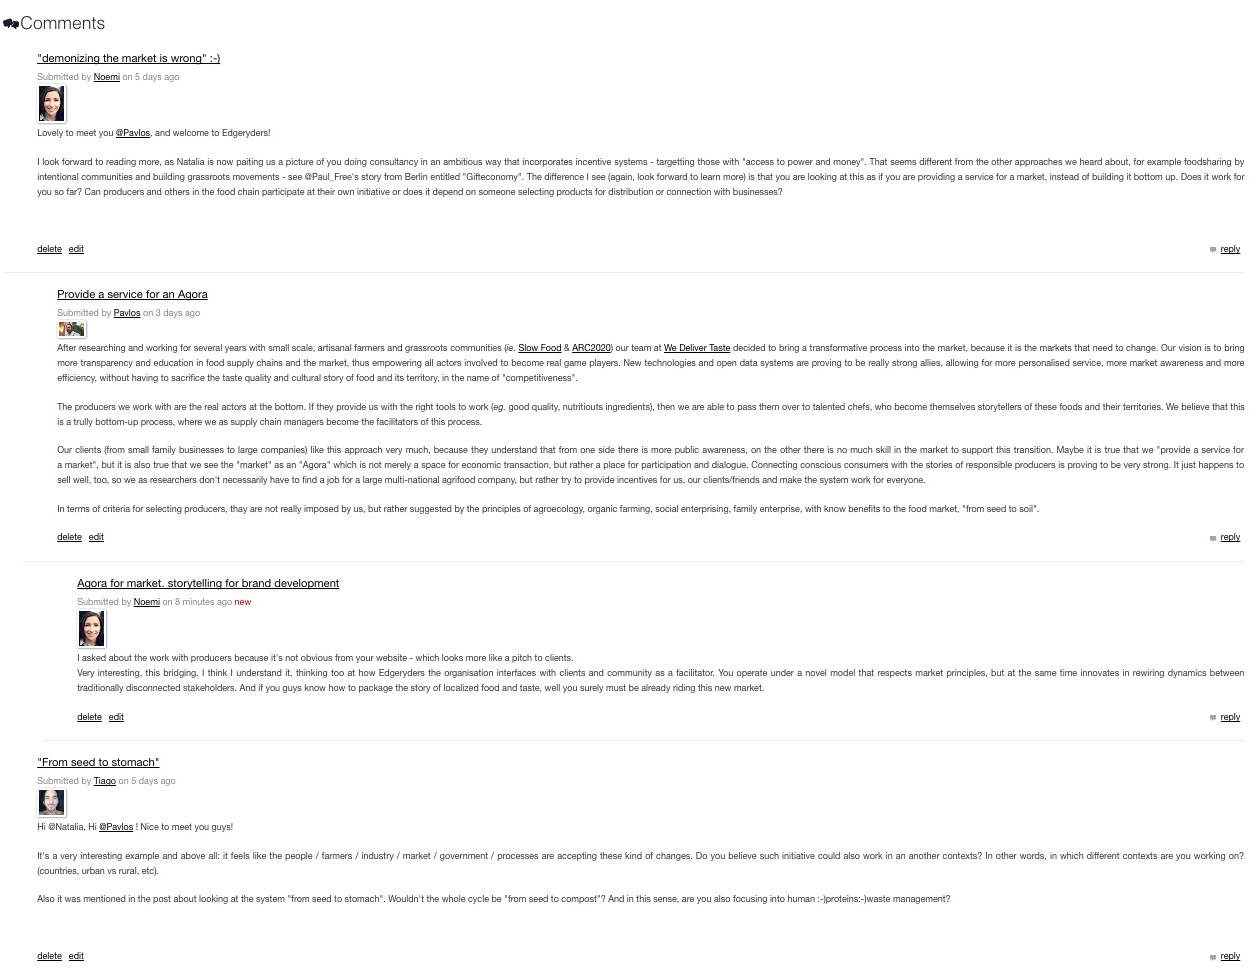
\includegraphics[width= 1 \textwidth]{Threaded_comments_Edgeryders}
	\caption{Threaded comments in the Edgeryders online community. Each comment is in turn commentable. This is represented visually by nested indentation: "sibling" comments (comments to the same post or comment) are visualized in chronological order, with the same level of indent. "Children" comments are visualized directly under their "parent", indented with respect to it.}
	\label{fig:threadedComments}
\end{figure}

We extracted a snapshot of the database on October 7th 2015. At the time, the community had 2,904 registered users, who had authored 4,062 posts and 18,285 comments. 23 of the users had, at some point in time, reported to the Edgeryders company; we cast them as the online community managers for this particular community. 	

All events in our dataset (creating accounts, creating posts, creating comments) are timestamped. This allows for the possibility of modelling interaction in the online community dynamically. 

\subsection{A network model of interaction in online communities}

We need to consider carefully how we incorporate dynamics in our model (\cite{holme2012temporal}). We make the following assumptions:

\begin{enumerate}
	\item The duration of interactions is negligible. This means that events can be represented by a contact sequence, i.e. triples $(i, j, t)$ where $i, j \in V$, the set of interactants (represented as vertices in the network) and $t$ denotes time. This is a standard assumption in studies of person-to-person communication online (\cite{holme2012temporal}). 
	\item First-time interaction produces a permanent change in the social relationship between the source and the target of the interaction (the author and the recipient of the comment). All Edgeryders users can be assumed to share some common interests around social innovation, that motivated them to join Edgeryders. When they interact directly, however, they begin to unpack and specify such common interests, and they (often explicitly) signal interest in each other's activities. This produces a shift in the nature of the relationship between the interacting, which becomes one of actual, as opposed to potential, interaction. Mathematically, this translates into representing interaction by a network whose edges do not decay.
	\item Subsequent interaction also carry social significance. They have the effect of further strengthening the relationship between the two interactants. The strength of the relationship increases monotonically with the number of interactions recorded. The effect of all  interactions after the first one, too, is permanent. Mathematically, this translates into representing interaction by a weighted network.
\end{enumerate}

We then proceeded to build a social network of the interactions within the community as follows:

\begin{enumerate}
	\item Users that have posted at least one post or one comment are included as nodes in the network.
	\item We interpret each comment as one interaction event. Whenever a comment is posted, an edge is induced. The new edge's source node is the node associated to the author of the comment. The new edge's target node is the node associated to the author of the post or comment being commented. 
	\item If an edge with the same source and target already exist, we do not add a new one, but rather increase the edge's weight by one.
	\item If the source and target of the edge are the same, the edge is discarded.  
	\item The sequence of timestamped interaction events allows us to model interaction in Edgeryders as an evolving network. We divide the observation period in one week-long intervals, and consider users to be acting on the basis of the interaction network that they find themselves in at that period. In other words, we do not attempt to model explicitly the entire sequence of interactions; rather, we assume that all agents make simultaneous decisions on who to interact with at the beginning of each time period, and that those decisions are based on the snapshot of the network at the beginning of said period. This means we are following the tradition of literature on evolving networks (\cite{dorogovtsev2002evolution}) rather than that of temporal networks (\cite{holme2012temporal}). This reflects our preoccupation with topological aspects over temporal ones. We claim the choice is justified under the terms suggested by Holme and Saramaki (\cite{holme2012temporal}) \footnote{" [...] a contact sequence that is fairly well modeled by a weighted graph with the assumption that contact times are random, with a frequency proportional to the edge weight"} .

\end{enumerate}

This process results in a sequence of 212 networks, each one a step on the growth path of the interaction network in Edgeryders. At the end of week 1 the network had only 6 nodes and 1 edge; at the end of week 212 it had 789 nodes and 4,861 edges.

\begin{figure}
	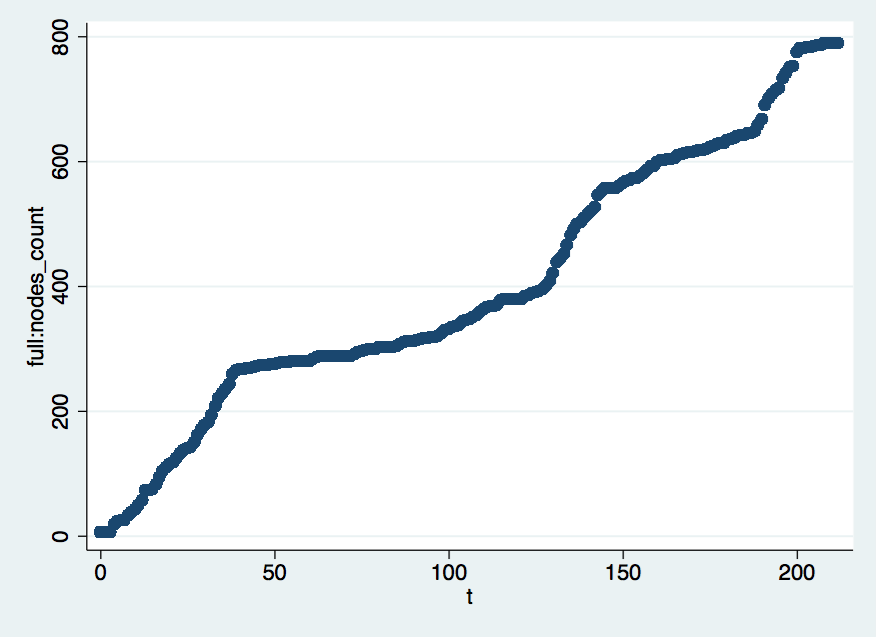
\includegraphics[width=.8 \textwidth]{numnodes}
	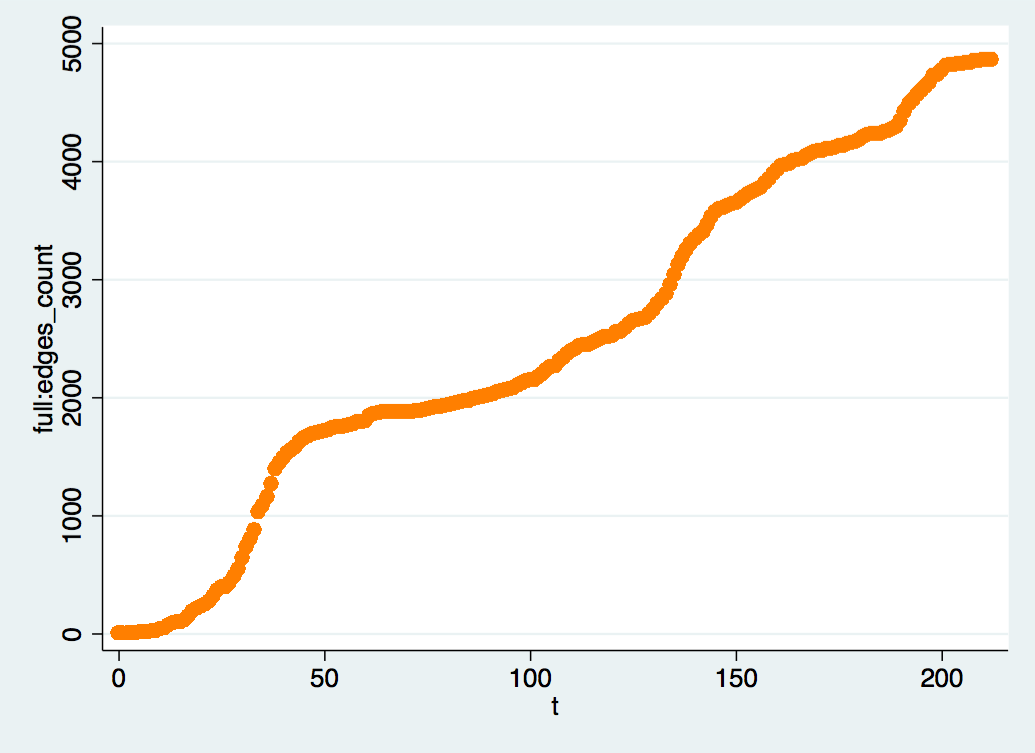
\includegraphics[width=.8 \textwidth]{numedges}
	\caption{Growth of the number of nodes (top) and edges (bottom) in the Edgeryders interaction network.}
\label{fig:growthNodesEdges}
\end{figure}

\subsection{Model}

We model user activity in an online community as a function of three groups of variables:

\begin{equation}
	A_{i,t} = f(NN_{i,t}, EN_{i,t}, GN_t) 
	\label{eq:model}
\end{equation}

Where:
\begin{itemize}
\item $A_{i,t}$ denotes the activity of user $i$ at time $t$, defined as the number of posts plus the number of comments authored by user $i$ during the period.
\item $NN_{i,t}$ denotes a vector of non-network variables associated with user $i$ at time $t$. These include writing a post or a comment; receiving a comment from a community manager; receiving a comment from another user who is not a community manager; the total number of posts and comments written by other users users $A_{j,t}, j \neq i$; and $i$'s experience as a user of Edgeryders, as measured by the number of weeks elapsed since she joined the community. The week of joining can predate the week in which the user writes her first post or comment. 
\item $EN_{i, t}$ denotes a vector of variables pertaining to the user's ego network at time $t$. These include her own in-degree (the number of users linking to her); her out-degree (the number of users she links to); her betweenness centrality (the fraction of shortest paths across any two users $j,k \neq i$ that $i$ finds herself on); her PageRank (the probability that a random walker across the network would end up at this particular node\footnote{PageRank was originally developed as a measure of network centrality for the World Wide Web (\cite{brin2012reprint}).}; and her clustering coefficient (the fraction of $i$'s neighbours that are also neighbours to each other).
\item $GN_{i,t}$ denotes a vector of variables pertaining to the global network at time $t$. These include the total number of nodes; the total number of edges; the average degree; and the network's Louvain modularity\footnote{The modularity of a network is a measure of how much it differs from an Erdos-Renyi random network with the same degree distribution. Values close to 0 indicate it is indistinguishable from a random network; values close to -1 or 1 indicate structure (\cite{clauset2004finding}). Measuring modularity is computationally hard; it is customary to use algorithms to compute an approximate value. Of these, the Louvain algorithm is the most widely used in the literature for its attractive computational efficiency \cite{blondel2008fast}.  }.
\end{itemize}

\subsection{Estimation}

We estimate the behaviour of a binary variable $A_{i,t}$ that takes value $1$ if user $i$ engages actively in interaction (i.e. writes a post or a comment at time $t$), and $0$ otherwise. We make use of a logit model:

\begin{equation}
	PR(A_{i,t}= 1|X_{i,t}) = \frac{e^{X_{i,t}\beta}}{1 + e^{X_{i,t}\beta}}
	\label{eq:estimation}
\end{equation}

Where $X_{i,t}$ is a vector of observed explanatory variables; $\beta$ is a vector of parameters.

An advantage of the logit model is that its coefficient lend themselves to being interpreted in terms of marginal effects on the log-odds ratio (\cite{cameron2005microeconometrics}). We rewrite equation \ref{eq:estimation} as

\begin{equation}
	ln \frac{Pr(A_{i,t} = 1)}{1 - Pr(A_{i,t}=1)} = X_{i,t} \beta 
	\label{eq:logOdds}
\end{equation}

Next, we proceed to estimating equation \ref{eq:logOdds} with fixed effects on the 766 Edgeryders users who have no moderator or site administrator role. To do this, we drop the 23 users that have such roles. We add to the right hand-side
$c_i$, an unobserved time-invariant effect specific to user $i$; this is intended to get rid of the bias introduced by different individuals having a different propensity to participate in the online conversation, as this is likely to be correlated with some of the regressors\footnote{For example, it is possible that "chattier" individuals might end up with higher in- and -out degrees, higher network centrality, and so on. }. We also add $u_{i,t}$, a residual error term, with mean zero and uncorrelated with right-hand side variables. We take care to employ lagged variables when failure to do so might cause endogeneity issues. 

\begin{equation}
	ln \frac{Pr(A_{i,t} = 1)}{1 - Pr(A_{i,t}=1)} = X_{i,t} \beta + c_i + u_{i,t}
	\label{eq:logOddsErrors}
\end{equation}

\subsection{Software stack}
Primary data from the Edgeryders database were obtained using a Drupal plugin called Views JSON. We used a modified version of an application software called Edgesense\footnote{https://github.com/Wikitalia/edgesense. Modifications added support for computing some extra network metrics, like the clustering coefficient.} to build a network representation of the interaction in Edgeryders. We then enriched the data so obtained with non-network metrics computed directly from the primary data, and exported the results in tabular form. Such results were then imported into Stata for estimation. 

 -\section{Results}

\subsection{Hypotheses}

We wish to test the following hypotheses.

\newtheorem{policyWorks}{Hypothesis}

\begin{policyWorks}
	The number of comments a user receives from community managers has no influence on her probability to be active.
	\label{hypothesis:policyWorks}
\end{policyWorks}

The organisations running online communities wish for their users to do certain things, most of which imply being active in the community itself: writing posts and comments. They cannot order them to do so, since users are not on the payroll and remain unanswerable to those organisations. Online community managers are then tasked to prompt users into action without using either monetary incentives or command power. That leaves interaction as the main tool online community managers have at their disposal. Rejecting Hypothesis \ref{hypothesis:policyWorks} would imply that users do, in fact, respond to cues from online community managers.

We expect Hypothesis \ref{hypothesis:policyWorks} to be falsified by data. Moreover, we expect that the coefficient on the number of comments received by the user from community managers, besides being statistically different from zero, is positive. Denote said coefficient by  $\beta_{cmrec}$, and the related variable by $x_{cmrec}$. Check that: 

\begin{equation}
	\frac{\partial Pr(A=1|x)}{\partial x_{cmrec}} > 0 \Rightarrow \frac{\partial LOR}{\partial x_{cmrec}} > 0
	\label{marginalProbActive}
\end{equation}

where $LOR$ denotes the logarithm of the log-odds ratio as per equation \ref{eq:logOddsErrors}. Since $x_{cmrec}$ enters equation \ref{eq:logOdds} linearly, equation \ref{marginalProbActive} implies that:

\begin{equation}
	\frac{\partial LOR}{\partial x_{cmrec}} > 0 \Rightarrow \beta_{cmrec} > 0 
\end {equation}

\begin{policyWorks}
	Receiving comments from community managers has the same effect on the probability to be active than receiving comments from users that are not community managers. 
	\label{hypothesis:policyWorksBetter}
\end{policyWorks}

Online community managers are professionals. They are likely to have better communication skills than the average user, and they certainly have stronger incentives to craft their interaction modes so as to drive users to being more active in the online community. We therefore expect, on average, the effect of incoming communication from online community manager to have a larger positive effect on the probability of becoming active than that of incoming communication from other users. Therefore, we expect Hypothesis \ref{hypothesis:policyWorksBetter} to be falsified by the data. 

\begin{policyWorks}
	Receiving an additional comment from a community manager has a large effect on the probability that a user becomes active. 	
	\label{hypothesis:policyWorksWell}
\end{policyWorks}

The number of comments authored by online community manager is the main policy variable in Edgeryders and other online communities like it. Employing community managers would not make economic sense if their impact on the level of activity in the community was not large enough. Hypothesis \ref{hypothesis:policyWorksWell} is more restrictive than Hypothesis \ref{hypothesis:policyWorks}, as it implies that the policy variable, the number of comments received from community manager, has a marginal effect that is not only statistically distinguishable from zero, but also sizeable. For example, if targeting users with a comment only increased their probability of being active by a few percent, many businesses running online communities would probably reconsider their decision to hire a community manager. 

\subsection{Regression}

Table \ref{tab:xtlogit} summarizes the estimation's results. 


\def\onepc{$^{\ast\ast}$} \def\fivepc{$^{\ast}$}
\def\tenpc{$^{\dag}$}
\def\legend{\multicolumn{4}{l}{\footnotesize{Significance levels
:\hspace{1em} $\dag$ : 10\% \hspace{1em}
$\ast$ : 5\% \hspace{1em} $\ast\ast$ : 1\% \normalsize}}}
\begin{table}[htbp]\centering
\begin{tabular}{l r @{} l c }\hline\hline 
\multicolumn{1}{c}
{\textbf{Variable}}
 & \multicolumn{2}{c}{\textbf{Coefficient}}  & \textbf{(Std. Err.)} \\ \hline
n. comments received from community managers  &  1.250&\onepc  & (0.053)\\
n. comments received from other users  &  0.215&\onepc  & (0.037)\\
n. comments and posts written by ego (lagged)  &  0.126&\tenpc  & (0.066)\\
weeks since creating the account  &  -0.011&\tenpc  & (0.006)\\
n. of posts and comments written by users excluding ego  &  0.037&\onepc  & (0.004)\\
n. of posts and comments written by community managers  &  0.001&  & (0.006)\\
user out-degree (lagged) &  0.028&\fivepc  & (0.013)\\
user in-degree (lagged)  &  -0.003&  & (0.013)\\
user betweenness centrality  &  -107.870&\onepc  & (20.778)\\
user pagerank (lagged) &  -5.592&  & (14.610)\\
user clustering coefficient  &  -0.654&\onepc  & (0.195)\\
network average distance  &  -4.156&\fivepc  & (2.007)\\
network average betweenness centrality at $t-1$  &  -9.260&  & (209.212)\\
network Louvain modularity  &  8.379&\onepc  & (2.520)\\
n. nodes  &  -0.001&  & (0.004)\\
n. edges  &  0.000&  & (0.001)\\
\hline
\onepc = 1\% significant; \fivepc = 5\% significant; \tenpc = 10\% significant.

\end{tabular}
 \caption{Estimation results for the dependent variable $A_{i,t}$}
\label{tab:xtlogit}
\end{table}


The coefficients on the first two variables are positive and highly significant ($p < 0.001$). This supports the conventional wisdom that users of online communities tend to engage with each other: when made the object of comments, they are more likely to become active than when they are not. By implication, our Hypothesis \ref{hypothesis:policyWorks} must be rejected. 

To test Hypothesis \ref{hypothesis:policyWorksBetter}, we start by noting that the coefficient on the number of comments received from community managers is larger than that on the number of comments received from other (non-community managers) users. We next run a Wald test on the null hypothesis that the coefficients on our first two variables are identical. The null is strongly rejected ($p < 0.0001$). This, in turn, means we have no support for Hypothesis \ref{hypothesis:policyWorksBetter}. 

Ideally, we would like that to support the alternative hypothesis that the difference between the coefficient on the number of comments received by the user from community managers and the coefficient on the number of comments received by other (non-community managers) users be positive. Wald tests, being one-tailed, cannot do that. However, we can deduce the non-negativity of such difference from the signs and values of the estimated coefficients and our functional form in equation \ref{eq:logOddsErrors}. Formally, denote the  coefficient on the number of comments received by other (non-community managers) users by $\beta_{urec}$, and the related variable by $x_{urec}$. Since the transformation from probability to odds is monotonic, we have:

\begin{equation}
	\frac{\partial Pr(A=1|x)}{\partial x_{cmrec}} > \frac{\partial Pr(A=1|x)}{\partial x_{urec}}  \Rightarrow \frac{\partial LOR}{\partial x_{cmrec}} > \frac{\partial LOR}{\partial x_{urec}} 
\end{equation}

Applying again equation \ref{eq:logOddsErrors}, and remembering that both $x_{cmrec}$ and $x_{urec}$ enter it linearly, we have:

\begin{equation}
	\frac{\partial LOR}{\partial x_{cmrec}} > \frac{\partial LOR}{\partial x_{urec}}\Rightarrow \beta_{cmrec} > \beta_{urec} \Rightarrow \beta_{cmrec} - \beta_{urec} > 0
	\label{eq:condition4WaldTest}
\end{equation}

So, the difference $\beta_{cmrec} - \beta_{urec}$ cannot be negative. Since we have strongly rejected that it be zero, it follows that it must be strictly positive. The activation effect of receiving comments from online community managers is thus significantly greater than that of receiving comments from ordinary users.

\subsection{Marginal effects}

Regression analysis shows that the activity of community managers does indeed have a positive impact on the probability that the users they engage will become active. This, however, does not tell us how large that impact is. Since online community management is costly, this is likely to be a question of some relevance to an organisation trying to make a decision to invest in it. 
Coefficient estimates are a poor indicator of marginal effects, because the logit model we employ here is not linear. The relationship between the linear prediction (as defined by the sum of each coefficient multiplied by the regressor it refers to, and assuming the fixed effects are zero) and the probability that the dependent variable is equal to 1 follows a logistic curve (figure \ref{fig:probActivityLinPredict}). An increase in the number of comments received by community managers has a small effect for small or large values of $x\beta$. When $x\beta$ is between -5 and 5, however, the probability that the user becomes active increases quickly as community managers engage more with the user.

\begin{figure}
	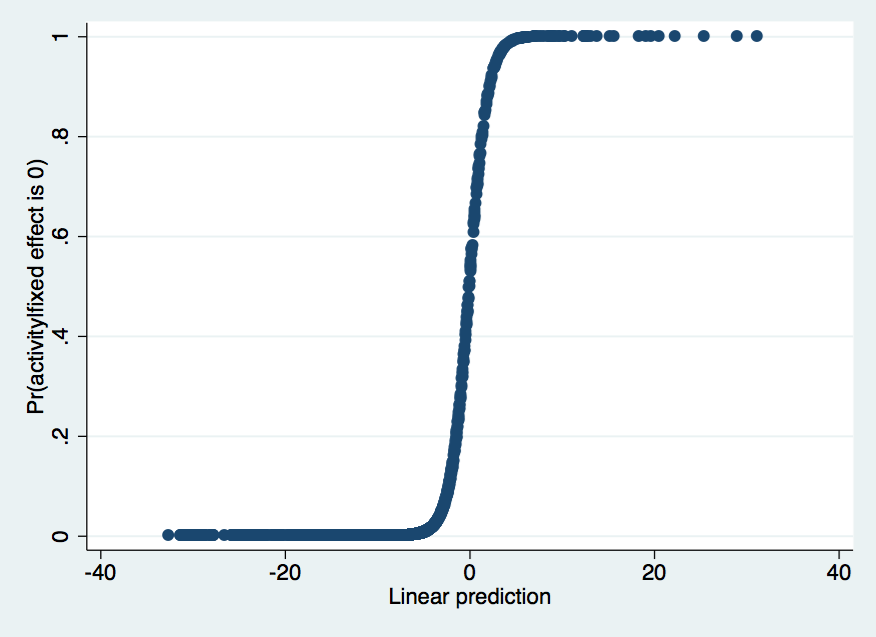
\includegraphics[width=.8 \textwidth]{PrAct_linPred}
	\caption{Predicted probability of Edgeryders users to become active as the linear prediction $x\beta$ based on number of comments received by community managers and other users increases.}
\label{fig:probActivityLinPredict}
\end{figure}

Table \ref{table:dydx} shows a point estimate the marginal effect of comments from the two sources (online community managers vs. other users) on the probability that a user will become active. Neither is significant. This turns out to be an artefact of the computation: the size of the marginal effect is computed fixing the value of regressors at their mean. The means of the variables in question are low. In the average period, the average Edgeryders user received 0.08 comments from online community managers and 0.09 comments from other users. This is consistent with what we know about patterns of human communication, which is sparse and bursty (\cite{holme2012temporal}). 

{
\def\onepc{$^{\ast\ast}$} \def\fivepc{$^{\ast}$}
\def\tenpc{$^{\dag}$}
\begin{table}[htbp]\centering
 \begin{tabular}{l c c c}\hline\hline 
\multicolumn{1}{c}
{\textbf{Variable}} & {\textbf{$dy/dx$}}  & \textbf{$Std. Err.$} & \textbf{$P > \lvert z \rvert$} \\ \hline
n. comments from community managers  &  .0000959  & .0004127 & 0.816 \\
n.  comments from other users  &  .0000165  & .000071 & 0.816\\
\hline
\end{tabular}
\caption{Marginal effects of the number of comments received by a user (both from community managers and from other users) on the probability of that user to become active. The estimates are computed under the assumption that regressors be fixed at their means. 
\label{table:dydx}}
\end{table}
}
A more intuitive approach is to estimate the elasticities of the probability of becoming active with respect to the number of comments received from each source. These are shown in table \ref{tab:elasticities}. They are both highly significant. In absolute terms, they are both small, but quite different. Receiving an extra comment by a community manager increases the probability that a user will become active by 10\%; but receiving one from another user will increase it by less than 2\%.

{
\def\onepc{$^{\ast\ast}$} \def\fivepc{$^{\ast}$}
\def\tenpc{$^{\dag}$}
\def\legend{\multicolumn{4}{l}{\footnotesize{Significance levels
:\hspace{1em} $\dag$ : 10\% \hspace{1em}
$\ast$ : 5\% \hspace{1em} $\ast\ast$ : 1\% \normalsize}}}
\begin{table}[htbp]\centering
 \begin{tabular}{l c c c}\hline\hline 
\multicolumn{1}{c}
{\textbf{Variable}} & {\textbf{$ey/ex$}}  & \textbf{$Std. Err.$} & \textbf{$P > \lvert z \rvert$} \\ \hline
n. comments from community managers  &  .1024245\onepc  & .0043113 & 0.000 \\
n. comments from other users  &  .01882\onepc  & .0032799 & 0.000\\
\hline
\end{tabular}
\caption{Elasticities of the probability that a user becomes active with respect to the number of comments received from community managers and from other users. The estimates are computed under the assumption that regressors be fixed at their means.
\label{tab:elasticities}}
\end{table}
}

Significant elasticities do not, per se, guarantee that the action of community managers will produce a large marginal effect in the online communities, unless the extra action (the differential increase in the regressor) is applied in a region of the distribution where the probability of the user being active is already reasonably high. We therefore turn to computing the marginal effect of the number of comments received from moderators on the probability that a user becomes active. Before we can proceed, however, we need an adjustment. In the model estimated so far, the mean of the predicted probability of a positive outcome (defined as the user
being active in the period) does not coincide with the proportion of users actually active across the dataset (table \ref{tab:flaw}). 

\begin{table}[htbp]\centering
 \begin{tabular}{l c c c}\hline\hline 
\multicolumn{1}{c}
{\textbf{Variable}} & {\textbf{Obs}}  & {\textbf{Mean}} & {\textbf{Std. Dev.}} \\ \hline
$prob$  &    84262   & .0023325  &  .0410453 \\
$active$  &  84262 &   .0181577  &  .1335221 \\
\hline
\end{tabular}\caption{Descriptive statistics for the probability of users to become active as predicted by the model ($prob$) and users actually being active ($active$).
\label{tab:flaw}}
\end{table}

This is caused by fact that the mean of the fixed effects $c_i$ in nonzero. To correct this, we need to add to the model a constant $\alpha$ such that: 

\begin{equation}
	 \frac{e^{mean(X_{i,t}\beta) + \alpha}}{1 + e^{mean(X_{i,t}\beta) + \alpha}} = \frac{\sum_{i = 1}^N \sum_{t = 1}^T active_{i,t}}{NT}
	 \label{eq:equationAlpha}
\end{equation}

In equation \ref{eq:equationAlpha}, $active_{1,t}$ takes value 1 if user $i$ is active at period $t$, and 0 otherwise; the $x_{i,t}\beta$ are the ones already estimated. The corrected model's linear predictions are unbiased, allowing us to compute marginal effects correctly. The right-hand side of equation \ref{eq:equationAlpha} is identical to the mean of the variable $active$ in table \ref{tab:flaw}. Replacing the appropriate values from table \ref{tab:flaw} yields:

\begin{equation}
	\frac{e^{-9.52 + \alpha}}{1 + e^{-9.52 + \alpha}} = 0.18
\end{equation}

\begin{equation}
	\alpha \simeq 8
	\label{eq:valueAlpha}
\end{equation}

We can now replace equation \ref{eq:valueAlpha} in to equation \ref{eq:equationAlpha} and proceed to estimate its marginal effects. Start by noting that, differentiating the right-hand side of \ref{eq:equationAlpha} with respect to $X$ yields:

\begin{equation}
	\frac{\partial Pr(A=1|X)}{\partial X} = \beta \frac{e^{X \beta + \alpha}}{(1 + e^{X \beta + \alpha})^2} 
\end{equation}

Replace the point estimates for $\beta_{cmrec}$, $\beta_{urec}$ and $\alpha$ to yield marginal effects of receiving one additional comments from, respectively, community managers and other users on the probability of being active in the period: 

\begin{equation}
	\frac{\partial Pr(A=1|X)}{\partial x_{cmrec}} = \beta_{cmrec} \frac{e^{ \beta_{cmrec} + \alpha}}{(1 + e^{x_{cmrec} \beta_{cmrec} + \alpha})^2} 
	\label{eq:marginal_x_cmrec}
\end{equation}

\begin{equation}
	\frac{\partial Pr(A=1|X)}{\partial x_{urec}} = \beta_{urec} \frac{e^{ \beta_{urec} + \alpha}}{(1 + e^{x_{urec} \beta_{urec} + \alpha})^2} 
	\label{eq:marginal_x_urec}
\end{equation}

Equations \ref{eq:marginal_x_cmrec} and \ref{eq:marginal_x_urec} allow us to "drill down" into the information contained in Table \ref{table:dydx} and study the marginal effects of receiving one additional comment after the same user has already received zero, one or more comments. To do so, we compute, for each observation and for both $x_{cmrec}$ and $x_{urec}$, the estimate of the marginal effect on the probability of the user being active. These are obtained plugging the observed regressor values, the computed value of $\alpha$ and the point estimates of the coefficient values into, respectively, equations \ref{eq:marginal_x_cmrec} and \ref{eq:marginal_x_urec}. We then repeat the procedure to compute the marginal effect of receiving comments from fellow participants in the Edgeryders community who are not online community managers. 

Plotting the frequency density of the two marginal effects shows that the comments of community managers have a greater activating marginal effect than those of non-community managers (Figure \ref{fig:marginalFxHisto}).

\begin{figure}
	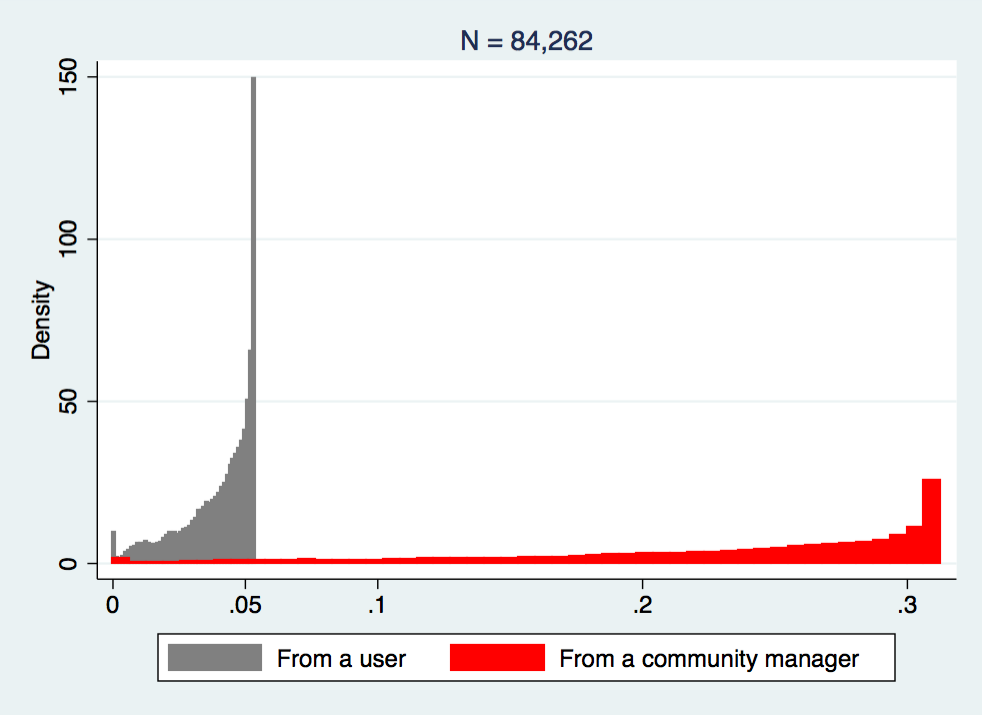
\includegraphics[width=.8 \textwidth]{Marginal_fx_histo}
	\caption{Frequency density of the marginal effect on the probability of being active of receiving a comment from online community managers and from other users in Edgeryders. Computed using point estimates for coefficient and observed values of regressors.}
\label{fig:marginalFxHisto}
\end{figure}

Marginal effects of regressors depend obviously on the values of regressors themselves. Receiving comments has generally decreasing returns on the probability of users becoming active. Fixing the value of all other regressors at their respective means and computing the marginal effects of both $x_{cmrec}$ and $x_{urec}$ as the number of comments received by users increase, we obtain the graph of Figure \ref{fig:marginalFxScat}. The marginal effect of $x{cmrec}$ is initially high (close to 0.3), but then decreases monotonically and quickly. That of $x{urec}$ starts at a much lower level (about 0.05), rises slightly to reach a maximum for $x{urec} = 2$, and then it decreases much more slowly.

\begin{figure}
	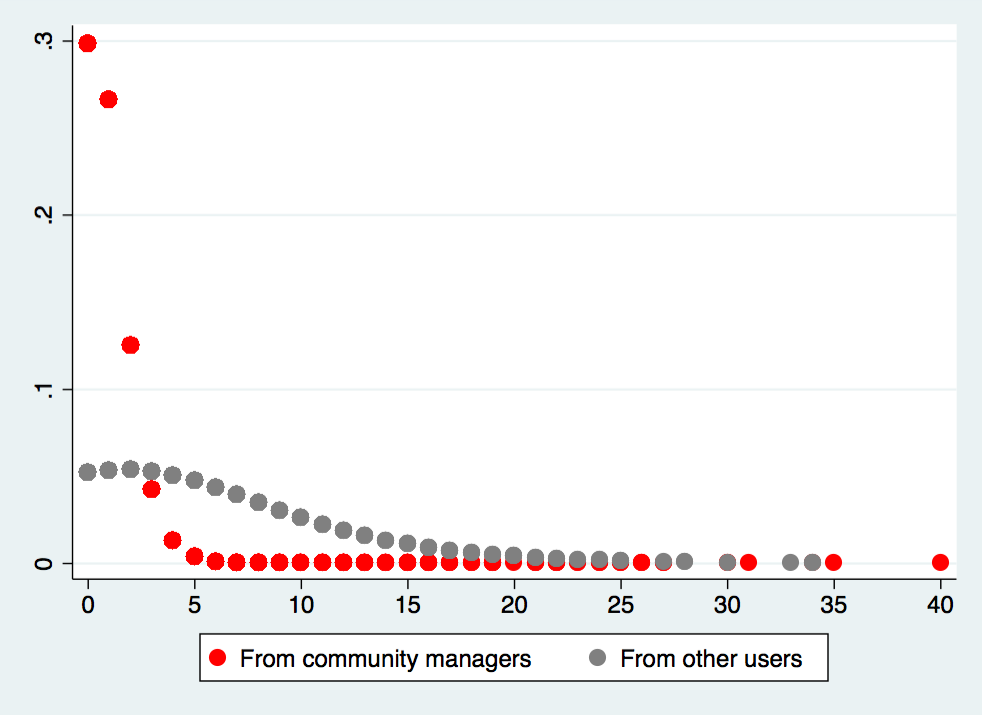
\includegraphics[width=.8 \textwidth]{Marginal_fx_scat}
	\caption{Marginal effect on the probability of being active of receiving a comment from online community managers and from other users in Edgeryders. Computed using point estimates for coefficient and mean values of regressors.}
\label{fig:marginalFxScat}
\end{figure}

This finding, illustrated by Figure \ref{fig:marginalFxScat} and Table \ref{tab:marginalProbabilityXcmrecObserved}, indicates support for Hypothesis \ref{hypothesis:policyWorksWell}, but only for low levels of $x_{cmrec}$.

Let's take a closer look, starting with the marginal effect of online community managers first. Tabulating the results according to the number of of comments received in each period by users, we derive Table \ref{tab:marginalProbabilityXcmrecObserved}. For users that have received no comments, the mass of the observations obtains for marginal probability values in or close to the 0.2-0.3 range. As the number of comments increases, predicted marginal probabilities decrease and quickly become indistinguishable from zero.

\begin{table}[htbp]\centering
	\begin{tabular}{c c | c  c  c  c | c}
 		& & \multicolumn{5}{c}{Marginal probability of user being active} \\
		& & \multicolumn{5}{c}{$X$ is at the observed value for each observation} \\
		\hline
		N. comments& & 0 - 0.1&0.1 - 0.2&0.2 - 0.3&over 0.3&Total \\
		\hline
		& mean & .06 & .15 & .26 & .31 & .23 \\ 
		0 & SE & .02 & .03 & .03 & .00 & .07 \\
		& N & 5,748&15,303&41,028&19,566&81,645 \\
		\hline
		 & mean & .04 & .14 & .25 & .31 & .15 \\
		1 & SE & .03 & .03 & .03 & .00 & .10 \\
		&N&438&308&362&111&1,219 \\
		\hline
		& mean & .03 & .14 & .25 & .31 & .07 \\
		2 & SE & .03 & . 03 & .03 & .00 & .08 \\
		& N&340&91&32&6&469 \\
		\hline
		& mean & .02 & .14 & . 25 & .31 & .04 \\
		3 & SE & .02 & .03 & .00 & .07 \\
		&N&223&8&13&2&246 \\
		\hline
		& mean & .01 & .12 & .25 & .31 & .04 \\
		4 & SE & .02 & .01 & .03 & .00 & .07 \\
		& N & 135 & 4 & 5 & 2 & 146 \\
		\hline
		& mean & .01 & .15 & .25 & .31 & .03 \\
		5 to 10 & SE & .02 & .03 &.03 & .00 & .08 \\
		& N&329&13&22&8&372 \\
		\hline
		& prob & .00 & .16 & .26 & .30 & .02 \\
		11 and above & SE & .01 & .03 & .04 & 0 & .05 \\
		& N &154&6&4&1&165 \\
		\hline
		& mean & .05 & .16 & .26 & .31 &.23 \\
		\textbf{Total} & SE & .03 & .03 & .03 & .00 & .08\\
		& N &7,367&15,733&41,466&19,696&84,262 \\
		\hline
	\end{tabular}
	\caption{Distribution of the observations according to the marginal effect of the user being active in the period with respect to receiving an extra comment from a community manager, and to the number of comments received in the same period. All other regressors enter the prediction function at the value observed for each observation.}

	\label{tab:marginalProbabilityXcmrecObserved}
\end{table}

Table \ref{tab:marginalProbabilityXcmrecObserved} has an interesting implication. The first and second comments any user receives are those with the highest (over .2) marginal effect on her activation in each period. Yet, community managers in Edgeryders write more than two comments to the same user in a relatively high number of instances. Of the 84,262 observations in our dataset, 2,617 are those for which the user received at least one comment from online community managers. Over a third (929) saw the user receiving three or more comments, having no predicted marginal effect on user activity in the period. We interpret these extra comments as exchanges, with community managers and users commenting (presumably) the same content within the same time period. This is not necessarily ineffective behaviour: online community managers might be driven by purposes other than activation, for example helping to give users a good experience of the community.  

We now turn to the marginal effect on the probability of being active of comments written by users who are not online community managers. Table \ref{tab:marginalProbabilityXurecObserved} is less informative than Table \ref{tab:marginalProbabilityXcmrecObserved}, given that the predicted marginal effect of $x_{urec}$ is smaller and more clustered around a single value than that of $x_{cmrec}$. Still, we do observe that the predicted marginal effect of the former is greater than .05 about one third of the times when $x_{urec} = 0$. As $x_{urec}$ increases, this proportion decreases, as does the average marginal effect.

\begin{table}[htbp]\centering
	\begin{tabular}{c c | c  c | c}
 		& & \multicolumn{3}{c}{Marginal probability of user being active} \\
		& & \multicolumn{3}{c}{$X$ is at the observed value for each observation} \\
		\hline
		N. comments& & 0 - 0.05&0.05 - 0.1&Total \\
		\hline
		& mean & .03 & .05 & .04 \\ 
		0 & SE & .01 & .00 & .01 \\
		& N & 56,183&25,716&81,899 \\
		\hline
		 & mean & .02 & .05 & .03 \\
		1 & SE & .02 & .00 & .02 \\
		&N&871 & 192 & 1,063 \\
		\hline
		& mean & .02 & .08 & .02 \\
		2 & SE & .02 & .00 &.02 \\
		& N& 425 & 47 & 472 \\
		\hline
		& mean & .01 & .05 & .01 \\
		3 & SE & .01 & .00 & .02 \\
		&N& 235 & 13 & 248\\
		\hline
		& mean & .01 & .05 & .01 \\
		4 & SE & .01 & .00 & .02 \\
		& N & 136 & 8 & 144 \\
		\hline
		& mean & .01 & .05 & .01  \\
		5 to 10 & SE & .01 & .00 & .01 \\
		& N&309&14& 323 \\
		\hline
		& prob & . & .00 \\
		11 and above & SE & .01 & . & .01\\
		& N &113 & 0 & 113\\
		\hline
		& mean & .03 & .05 & .04 \\
		\textbf{Total} & SE & .01 & .00 & .01\\
		& N & 58,272 & 25,990 & 84262 \\
		\hline
	\end{tabular}
	\caption{Distribution of the observations according to the marginal effect of the user being active in the period with respect to receiving an extra comment from a non-community manager, and to the number of comments received in the same period. All other regressors enter the prediction function at the value observed for each observation.}
	\label{tab:marginalProbabilityXurecObserved}
\end{table}


 -\section{Discussion}

The existence of professional online community managers is predicated on their work solving some optimisation problem for organisations running the online community themselves. Their ability to do so rests ultimately on the influence they can exert on the other participants in the online community. Given the pervasiveness of online community management as a profession, it is perhaps surprising that this influence is generally simply assumed to be there: we have been unable to find explicit empirical tests that this assumption is correct. In this paper, we devise an econometric test for it, and implement it on one online community, called Edgeryders, that explicitly relies on community management as a way to get more, better engagement from its members. We find that interaction with online community managers is associated with a measurably higher probability of users in the online community becoming active. 

We also find that interaction with other (non-community managers) users also increases a user's probability of becoming active; but that this increase is significantly smaller than that associated with the interaction with online community managers. We interpret this as the signature of of the latter's professional skills. 

Our data lend some support to those authors who claim that the topology of the interaction network in online communities influences user behaviour. The probability of a user becoming active depends on some ego network variables (clustering coefficient and betweenness centrality, negatively for both variables) and one global network variable (Louvain modularity, positively) in statistically significant ways. Furthermore, incoming communication is effective in prompting additional (outgoing) communication. This is consistent with the "bursty" nature of human communication described in section \ref{Literature survey}.

In a previous paper (\cite{cottica2015online}), we built a simulation model around the assumption that online community managers could influence the behaviour of other users. That paper makes use of a scalar parameter representing the effectiveness of the community management policy ("onboarding effectiveness"), represented as the increase in probability that users would become active conditional to receiving a communication from one of the community managers. That paper makes no attempt to provide a plausible value for that probability, letting it vary between 0 and 1. The policy considered there is the same as that considered here, except that in \cite{cottica2015online} it targets only newcomers to the online community. Nevertheless, if we are prepared to assume that the propensity to respond to receiving comments to one's content does not change after one's very first contribution to an online community, we can use the data in this paper to attempt a quantification of the onboarding effectiveness parameter. In Edgeryders, the value of the policy effectiveness parameter could be estimated at starting in the 0.2 to 0.3 range, rapidly decreasing as the number of comments received increases. We also computed the marginal effect of receiving comments from users who are not online community managers, and that can be used as an estimate for the second parameter used in \cite{cottica2015online} ("community responsiveness"). We found it to be starting around 0.05, slowly decreasing as the number of comments received increases. 
 -
 -\appendices
 -
 -\input{appendix.tex}
 -
 -\section*{Acknowledgements}
 -The authors gratefully acknowledge the invaluable contributions of Giovanni Ponti, Raffaele Miniaci, Noemi Salantiu, Lee-Sean Huang, the faculty and students at University of Alicante and everybody at Masters of Networks 3.
 -
 -%Alberto Cottica %maybe for blind review?
 -The authors acknowledges the support of the CATALYST European project in developing the Edgesense tool and acting as a conversation starter between the collective intelligence and the network science research communities.

% Can use something like this to put references on a page
% by themselves when using endfloat and the captionsoff option.
\ifCLASSOPTIONcaptionsoff
  \newpage
\fi



% trigger a \newpage just before the given reference
% number - used to balance the columns on the last page
% adjust value as needed - may need to be readjusted if
% the document is modified later
%\IEEEtriggeratref{8}
% The "triggered" command can be changed if desired:
%\IEEEtriggercmd{\enlargethispage{-5in}}

% references section

-\bibliographystyle{IEEEtran}
 -\bibliography{bibliography}
% biography section
% 
% If you have an EPS/PDF photo (graphicx package needed) extra braces are
% needed around the contents of the optional argument to biography to prevent
% the LaTeX parser from getting confused when it sees the complicated
% \includegraphics command within an optional argument. (You could create
% your own custom macro containing the \includegraphics command to make things
% simpler here.)
%\begin{IEEEbiography}[{\includegraphics[width=1in,height=1.25in,clip,keepaspectratio]{mshell}}]{Michael Shell}
% or if you just want to reserve a space for a photo:

%\begin{IEEEbiography}{Michael Shell}
%Biography text here.
%\end{IEEEbiography}

% if you will not have a photo at all:
%\begin{IEEEbiographynophoto}{John Doe}
%Biography text here.
%\end{IEEEbiographynophoto}

% insert where needed to balance the two columns on the last page with
% biographies
%\newpage

%\begin{IEEEbiographynophoto}{Jane Doe}
%Biography text here.
%\end{IEEEbiographynophoto}

% You can push biographies down or up by placing
% a \vfill before or after them. The appropriate
% use of \vfill depends on what kind of text is
% on the last page and whether or not the columns
% are being equalized.

%\vfill

% Can be used to pull up biographies so that the bottom of the last one
% is flush with the other column.
%\enlargethispage{-5in}



% that's all folks
\end{document}


